\documentclass {article}

\usepackage{graphicx}

\title {Introduction to JavaScript}


\begin{document}

\maketitle

\section {History}

\begin{itemize}
	\item Created at Netscape
	\item Originally written in 1995 by Brandon Eich
	\item Called JavaScript to entice Java developers to try it
	\item Microsoft reverse engineered the language for integration into Internet Explorertext
	\item Become ECMA Script in 1997 and is when Netscape lost control. 
\end{itemize}


\section{Coding Standards}
	\subsection{JsLint}
		Before programming download and install JSLint.  There is an addon to Visual Studio under: 
		
		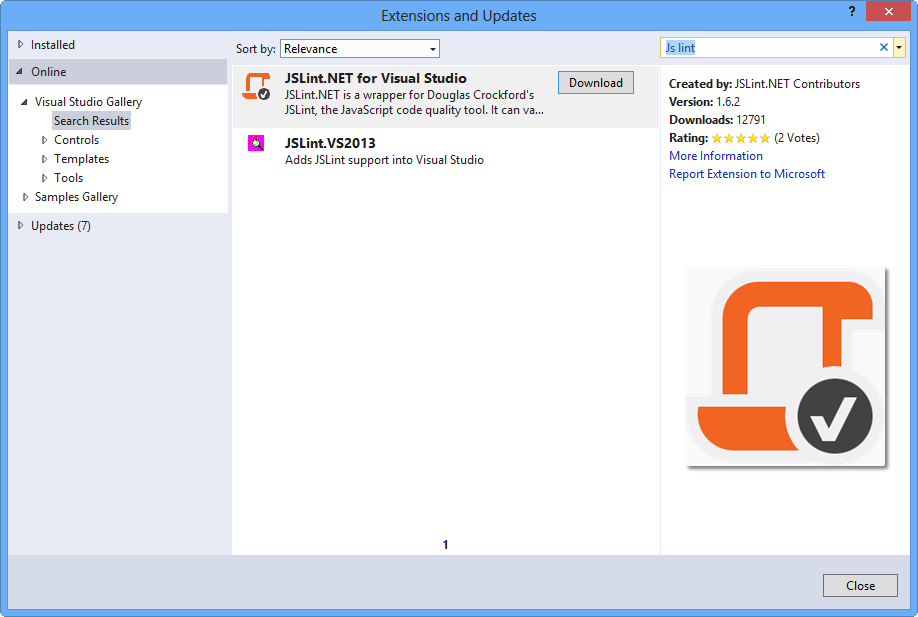
\includegraphics[scale=.25]{JsLintAddOn.png}

\section{Statement Endings}
	\subsection{Semicolons}
		This is the optimal way of ending a statement.  Always use this.
	\subsection {Carriage Return}
		A carriage return will end a statement.  This happens by JavaScript inserting a semicolon when it encounters an error.  If this corrects the error, then JavaScript assumes that not having a semicolon was the cause and continues on. 


\section{Operators}
	\subsection{=== and !==}
		This is the actual comparison operator.  This acts like == in other langauges.
	\subsection{== and !=}
		This does the object on the right hand side of the operator convert to the left.  
		Consider the following: 

		\begin{itemize}
			\item "" == "0" //false
			\item 0 == '' //true
			\item 0 == '0' //true
		\end{itemize}

		\n

		\begin{itemize}
			\item false == 'false' //false
			\item false == '0' //true
		\end{itemize}

		\n

		\begin{itemize}
			\item false == undefined //false
			\item false == null //false
			\item null == undefined //true
			\item ' \textbackslash{t} \textbackslash{r} \textbackslash{n} ' == 0 //true
		\end{itemize}

\section{Variables}

\section{Functions}
	There are 3 ways to create a function: 
	\begin{itemize}
		\item function foo () /{/}
		\item var foo = function () /{/}
		\item function () /{/} //anonymous
	\end{itemize}


\section{Primitive Types}
	\subsection{Strings}
			\subsection{Escape Characters}

			\begin{center}
			\begin{tabular} {| l |p{5cm}|}
			
				\textbackslash{b} & Backspace \\
				\textbackslash{t} & Tab (horizontal) \\
				\textbackslash{n} & Linefeed (newline) \\
				\textbackslash{v} & Tab (vertical) \\
				\textbackslash{f} & Form feed  \\
				\textbackslash{r} & Carriage return        \\
				\textbackslash{"} & Double quote           \\
				\textbackslash{'} & Single quote           \\
				\textbackslash{}\textbackslash{} & Backslash              \\

			\end{tabular}
			\end{center}
\subsection{number}
	All numbers in JavaScript are 64-bit floating point numbers.
\subsection {undefined}
\subsection {null}


\section{Objects}
	\subsection {Reference Types}
		In JavaScript everything is an object, and all objects are reference types.  There is no pass by value in JavaScript.  
		What this means: 
	
	\subsection{Creating an Object}
		\begin{itemize}
			\item Literal Notation: var o = \{\};
			\item Function: var o = new Object();
		\end{itemize}		

	\subsection{Arrays}
		\subsubsection {Creating an Array}
			\begin{itemize}
				\item Literal Notation: var arr = [];
				\item Function: var o = new Array();
			\end{itemize}
	
	

			

\end{document}